% Options for packages loaded elsewhere
% Options for packages loaded elsewhere
\PassOptionsToPackage{unicode}{hyperref}
\PassOptionsToPackage{hyphens}{url}
\PassOptionsToPackage{dvipsnames,svgnames,x11names}{xcolor}
%
\documentclass[
  letterpaper,
  DIV=11,
  numbers=noendperiod]{scrartcl}
\usepackage{xcolor}
\usepackage{amsmath,amssymb}
\setcounter{secnumdepth}{-\maxdimen} % remove section numbering
\usepackage{iftex}
\ifPDFTeX
  \usepackage[T1]{fontenc}
  \usepackage[utf8]{inputenc}
  \usepackage{textcomp} % provide euro and other symbols
\else % if luatex or xetex
  \usepackage{unicode-math} % this also loads fontspec
  \defaultfontfeatures{Scale=MatchLowercase}
  \defaultfontfeatures[\rmfamily]{Ligatures=TeX,Scale=1}
\fi
\usepackage{lmodern}
\ifPDFTeX\else
  % xetex/luatex font selection
\fi
% Use upquote if available, for straight quotes in verbatim environments
\IfFileExists{upquote.sty}{\usepackage{upquote}}{}
\IfFileExists{microtype.sty}{% use microtype if available
  \usepackage[]{microtype}
  \UseMicrotypeSet[protrusion]{basicmath} % disable protrusion for tt fonts
}{}
\makeatletter
\@ifundefined{KOMAClassName}{% if non-KOMA class
  \IfFileExists{parskip.sty}{%
    \usepackage{parskip}
  }{% else
    \setlength{\parindent}{0pt}
    \setlength{\parskip}{6pt plus 2pt minus 1pt}}
}{% if KOMA class
  \KOMAoptions{parskip=half}}
\makeatother
% Make \paragraph and \subparagraph free-standing
\makeatletter
\ifx\paragraph\undefined\else
  \let\oldparagraph\paragraph
  \renewcommand{\paragraph}{
    \@ifstar
      \xxxParagraphStar
      \xxxParagraphNoStar
  }
  \newcommand{\xxxParagraphStar}[1]{\oldparagraph*{#1}\mbox{}}
  \newcommand{\xxxParagraphNoStar}[1]{\oldparagraph{#1}\mbox{}}
\fi
\ifx\subparagraph\undefined\else
  \let\oldsubparagraph\subparagraph
  \renewcommand{\subparagraph}{
    \@ifstar
      \xxxSubParagraphStar
      \xxxSubParagraphNoStar
  }
  \newcommand{\xxxSubParagraphStar}[1]{\oldsubparagraph*{#1}\mbox{}}
  \newcommand{\xxxSubParagraphNoStar}[1]{\oldsubparagraph{#1}\mbox{}}
\fi
\makeatother

\usepackage{color}
\usepackage{fancyvrb}
\newcommand{\VerbBar}{|}
\newcommand{\VERB}{\Verb[commandchars=\\\{\}]}
\DefineVerbatimEnvironment{Highlighting}{Verbatim}{commandchars=\\\{\}}
% Add ',fontsize=\small' for more characters per line
\usepackage{framed}
\definecolor{shadecolor}{RGB}{241,243,245}
\newenvironment{Shaded}{\begin{snugshade}}{\end{snugshade}}
\newcommand{\AlertTok}[1]{\textcolor[rgb]{0.68,0.00,0.00}{#1}}
\newcommand{\AnnotationTok}[1]{\textcolor[rgb]{0.37,0.37,0.37}{#1}}
\newcommand{\AttributeTok}[1]{\textcolor[rgb]{0.40,0.45,0.13}{#1}}
\newcommand{\BaseNTok}[1]{\textcolor[rgb]{0.68,0.00,0.00}{#1}}
\newcommand{\BuiltInTok}[1]{\textcolor[rgb]{0.00,0.23,0.31}{#1}}
\newcommand{\CharTok}[1]{\textcolor[rgb]{0.13,0.47,0.30}{#1}}
\newcommand{\CommentTok}[1]{\textcolor[rgb]{0.37,0.37,0.37}{#1}}
\newcommand{\CommentVarTok}[1]{\textcolor[rgb]{0.37,0.37,0.37}{\textit{#1}}}
\newcommand{\ConstantTok}[1]{\textcolor[rgb]{0.56,0.35,0.01}{#1}}
\newcommand{\ControlFlowTok}[1]{\textcolor[rgb]{0.00,0.23,0.31}{\textbf{#1}}}
\newcommand{\DataTypeTok}[1]{\textcolor[rgb]{0.68,0.00,0.00}{#1}}
\newcommand{\DecValTok}[1]{\textcolor[rgb]{0.68,0.00,0.00}{#1}}
\newcommand{\DocumentationTok}[1]{\textcolor[rgb]{0.37,0.37,0.37}{\textit{#1}}}
\newcommand{\ErrorTok}[1]{\textcolor[rgb]{0.68,0.00,0.00}{#1}}
\newcommand{\ExtensionTok}[1]{\textcolor[rgb]{0.00,0.23,0.31}{#1}}
\newcommand{\FloatTok}[1]{\textcolor[rgb]{0.68,0.00,0.00}{#1}}
\newcommand{\FunctionTok}[1]{\textcolor[rgb]{0.28,0.35,0.67}{#1}}
\newcommand{\ImportTok}[1]{\textcolor[rgb]{0.00,0.46,0.62}{#1}}
\newcommand{\InformationTok}[1]{\textcolor[rgb]{0.37,0.37,0.37}{#1}}
\newcommand{\KeywordTok}[1]{\textcolor[rgb]{0.00,0.23,0.31}{\textbf{#1}}}
\newcommand{\NormalTok}[1]{\textcolor[rgb]{0.00,0.23,0.31}{#1}}
\newcommand{\OperatorTok}[1]{\textcolor[rgb]{0.37,0.37,0.37}{#1}}
\newcommand{\OtherTok}[1]{\textcolor[rgb]{0.00,0.23,0.31}{#1}}
\newcommand{\PreprocessorTok}[1]{\textcolor[rgb]{0.68,0.00,0.00}{#1}}
\newcommand{\RegionMarkerTok}[1]{\textcolor[rgb]{0.00,0.23,0.31}{#1}}
\newcommand{\SpecialCharTok}[1]{\textcolor[rgb]{0.37,0.37,0.37}{#1}}
\newcommand{\SpecialStringTok}[1]{\textcolor[rgb]{0.13,0.47,0.30}{#1}}
\newcommand{\StringTok}[1]{\textcolor[rgb]{0.13,0.47,0.30}{#1}}
\newcommand{\VariableTok}[1]{\textcolor[rgb]{0.07,0.07,0.07}{#1}}
\newcommand{\VerbatimStringTok}[1]{\textcolor[rgb]{0.13,0.47,0.30}{#1}}
\newcommand{\WarningTok}[1]{\textcolor[rgb]{0.37,0.37,0.37}{\textit{#1}}}

\usepackage{longtable,booktabs,array}
\newcounter{none} % for unnumbered tables
\usepackage{calc} % for calculating minipage widths
% Correct order of tables after \paragraph or \subparagraph
\usepackage{etoolbox}
\makeatletter
\patchcmd\longtable{\par}{\if@noskipsec\mbox{}\fi\par}{}{}
\makeatother
% Allow footnotes in longtable head/foot
\IfFileExists{footnotehyper.sty}{\usepackage{footnotehyper}}{\usepackage{footnote}}
\makesavenoteenv{longtable}
\usepackage{graphicx}
\makeatletter
\newsavebox\pandoc@box
\newcommand*\pandocbounded[1]{% scales image to fit in text height/width
  \sbox\pandoc@box{#1}%
  \Gscale@div\@tempa{\textheight}{\dimexpr\ht\pandoc@box+\dp\pandoc@box\relax}%
  \Gscale@div\@tempb{\linewidth}{\wd\pandoc@box}%
  \ifdim\@tempb\p@<\@tempa\p@\let\@tempa\@tempb\fi% select the smaller of both
  \ifdim\@tempa\p@<\p@\scalebox{\@tempa}{\usebox\pandoc@box}%
  \else\usebox{\pandoc@box}%
  \fi%
}
% Set default figure placement to htbp
\def\fps@figure{htbp}
\makeatother





\setlength{\emergencystretch}{3em} % prevent overfull lines

\providecommand{\tightlist}{%
  \setlength{\itemsep}{0pt}\setlength{\parskip}{0pt}}



 


\KOMAoption{captions}{tableheading}
\makeatletter
\@ifpackageloaded{tcolorbox}{}{\usepackage[skins,breakable]{tcolorbox}}
\@ifpackageloaded{fontawesome5}{}{\usepackage{fontawesome5}}
\definecolor{quarto-callout-color}{HTML}{909090}
\definecolor{quarto-callout-note-color}{HTML}{0758E5}
\definecolor{quarto-callout-important-color}{HTML}{CC1914}
\definecolor{quarto-callout-warning-color}{HTML}{EB9113}
\definecolor{quarto-callout-tip-color}{HTML}{00A047}
\definecolor{quarto-callout-caution-color}{HTML}{FC5300}
\definecolor{quarto-callout-color-frame}{HTML}{acacac}
\definecolor{quarto-callout-note-color-frame}{HTML}{4582ec}
\definecolor{quarto-callout-important-color-frame}{HTML}{d9534f}
\definecolor{quarto-callout-warning-color-frame}{HTML}{f0ad4e}
\definecolor{quarto-callout-tip-color-frame}{HTML}{02b875}
\definecolor{quarto-callout-caution-color-frame}{HTML}{fd7e14}
\makeatother
\makeatletter
\@ifpackageloaded{caption}{}{\usepackage{caption}}
\AtBeginDocument{%
\ifdefined\contentsname
  \renewcommand*\contentsname{Table of contents}
\else
  \newcommand\contentsname{Table of contents}
\fi
\ifdefined\listfigurename
  \renewcommand*\listfigurename{List of Figures}
\else
  \newcommand\listfigurename{List of Figures}
\fi
\ifdefined\listtablename
  \renewcommand*\listtablename{List of Tables}
\else
  \newcommand\listtablename{List of Tables}
\fi
\ifdefined\figurename
  \renewcommand*\figurename{Figure}
\else
  \newcommand\figurename{Figure}
\fi
\ifdefined\tablename
  \renewcommand*\tablename{Table}
\else
  \newcommand\tablename{Table}
\fi
}
\@ifpackageloaded{float}{}{\usepackage{float}}
\floatstyle{ruled}
\@ifundefined{c@chapter}{\newfloat{codelisting}{h}{lop}}{\newfloat{codelisting}{h}{lop}[chapter]}
\floatname{codelisting}{Listing}
\newcommand*\listoflistings{\listof{codelisting}{List of Listings}}
\makeatother
\makeatletter
\makeatother
\makeatletter
\@ifpackageloaded{caption}{}{\usepackage{caption}}
\@ifpackageloaded{subcaption}{}{\usepackage{subcaption}}
\makeatother
\usepackage{bookmark}
\IfFileExists{xurl.sty}{\usepackage{xurl}}{} % add URL line breaks if available
\urlstyle{same}
\hypersetup{
  pdftitle={Lab 1 Instructions},
  pdfauthor={Nicky Wakim},
  colorlinks=true,
  linkcolor={blue},
  filecolor={Maroon},
  citecolor={Blue},
  urlcolor={Blue},
  pdfcreator={LaTeX via pandoc}}


\title{Lab 1 Instructions}
\usepackage{etoolbox}
\makeatletter
\providecommand{\subtitle}[1]{% add subtitle to \maketitle
  \apptocmd{\@title}{\par {\large #1 \par}}{}{}
}
\makeatother
\subtitle{PUBH 523/623}
\author{Nicky Wakim}
\date{}
\begin{document}
\maketitle


\subsection{Directions}\label{directions}

\href{https://github.com/nwakim/BSTA_513_26S/blob/main/project/LastName_FirstInit_Lab_01.qmd}{You
can download the \texttt{.qmd} file for this lab here.}

The above link will take you to your \textbf{editing} file.
\textbf{Please do not remove anything from this editing file!!} You will
only add your code and work to this file.

\subsection{Lab activities}\label{lab-activities}

\subsubsection{Familiarize yourself with the Well-Being and Basic Needs
Survey}\label{familiarize-yourself-with-the-well-being-and-basic-needs-survey}

Please read the
\href{https://www.urban.org/policy-centers/health-policy-center/projects/well-being-and-basic-needs-survey}{Urban
Institute's page} on the Well-Being and Basic Needs Survey (WBNS) and
more of their
\href{https://www.urban.org/sites/default/files/publication/98919/the_well-being_and_basic_needs_survey_1.pdf}{published
information of the survey} (at least the first 4 pages). You can also
read about the overarching
\href{https://www.urban.org/tags/safety-net-solid-ground\#about}{From
Safety Net to Solid Ground Initiative} that started the survey. Answer
the following questions:

\begin{itemize}
\tightlist
\item
  What is the motivation for this study?
\item
  How could an analysis that looks at associations with food insecurity
  help facilitate change in policy?
\item
  Why is it important to study food insecurity?
\end{itemize}

\begin{tcolorbox}[enhanced jigsaw, arc=.35mm, bottomrule=.15mm, bottomtitle=1mm, breakable, colback=white, colbacktitle=quarto-callout-important-color!10!white, colframe=quarto-callout-important-color-frame, coltitle=black, left=2mm, leftrule=.75mm, opacityback=0, opacitybacktitle=0.6, rightrule=.15mm, title=\textcolor{quarto-callout-important-color}{\faExclamation}\hspace{0.5em}{Task}, titlerule=0mm, toprule=.15mm, toptitle=1mm]

Answer the following questions using information on WBNS:

\begin{itemize}
\tightlist
\item
  What is the motivation for this study?
\item
  How could an analysis that looks at associations with food insecurity
  help facilitate change in policy?
\item
  Why is it important to study food insecurity?
\end{itemize}

\end{tcolorbox}

\subsubsection{File organization}\label{file-organization}

Before downloading the data, set up your folders for the class and
project, including making an \texttt{.Rproj} file. Make sure you are
working with the project by using the \texttt{here()} function to
display your working directory.

\begin{tcolorbox}[enhanced jigsaw, arc=.35mm, bottomrule=.15mm, bottomtitle=1mm, breakable, colback=white, colbacktitle=quarto-callout-important-color!10!white, colframe=quarto-callout-important-color-frame, coltitle=black, left=2mm, leftrule=.75mm, opacityback=0, opacitybacktitle=0.6, rightrule=.15mm, title=\textcolor{quarto-callout-important-color}{\faExclamation}\hspace{0.5em}{Task}, titlerule=0mm, toprule=.15mm, toptitle=1mm]

Display your working directory using the \texttt{here} package and
\texttt{here()} function.

Insert an image of your folder organization with the \texttt{.Rproj}
file in the correct place.

\end{tcolorbox}

\subsubsection{Access and download the
data}\label{access-and-download-the-data}

\begin{enumerate}
\def\labelenumi{\arabic{enumi}.}
\tightlist
\item
  Go to the
  \href{https://www.icpsr.umich.edu/web/HMCA/studies/39691/datadocumentation}{Health
  and Medical Care Archive page for the 2024 Well-Being and Basic Needs
  Survey}
\item
  Go to the Data \& Documentation tab
  \pandocbounded{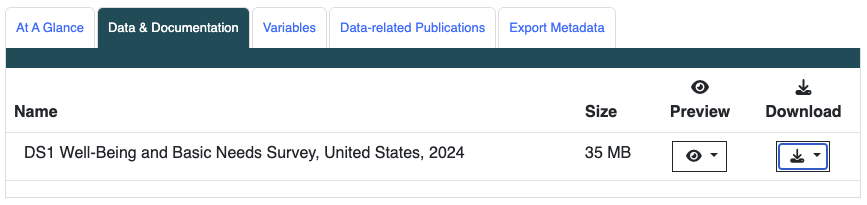
\includegraphics[keepaspectratio]{./images/Lab_01/dnd.png}}
\item
  Download the R version of the Public use data
  \pandocbounded{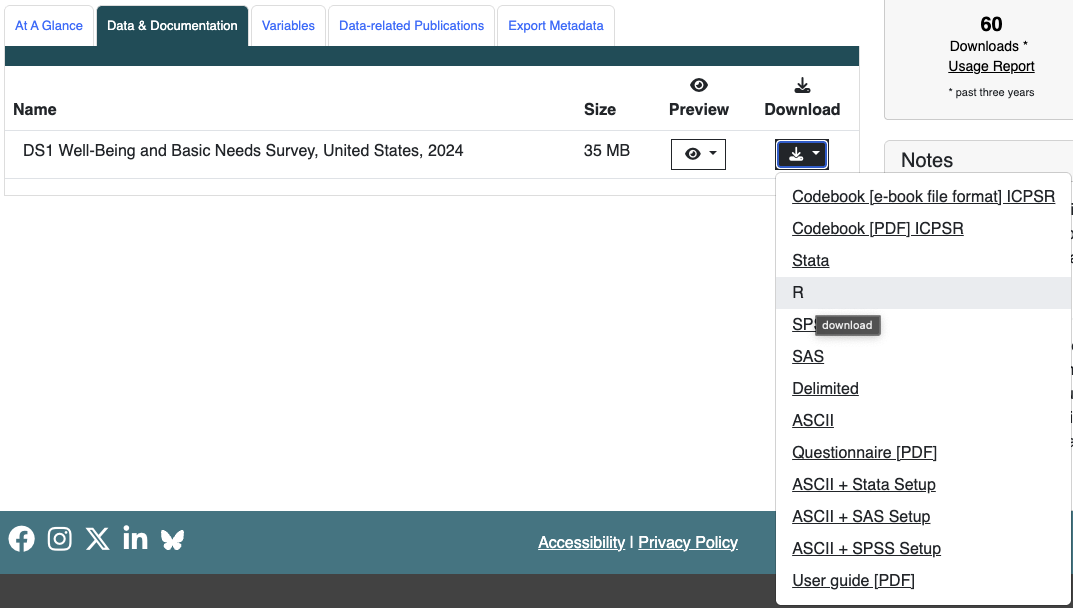
\includegraphics[keepaspectratio]{./images/Lab_01/download.png}}
\item
  Read and agree to the Terms of Use. After this, you will be redirected
  to a new page.
\item
  Log into ICPSR by clicking ``Access through your institution''. You
  should be taken to a new page where you need to select ``Oregon Health
  \& Science University''
  \pandocbounded{
\includegraphics[keepaspectratio]{./images/Lab_01/ICPSR.png}}
\item
  Login using standard OHSU login. Then the download should begin!
\item
  Make sure to move this into your project folder under the ``data''
  folder.
\item
  Take a look at the folders/files you just downloaded. Make sure to
  locate and understand the difference between the Codebook,
  Questionnaire, and User Guide. (Note that the website also contains
  the codebook if you go to the variable tab. I think the online one has
  an easier user interface than the pdf.)
\item
  \textbf{Read the User Guide!} There is some important information
  about the data and how to use it.
\end{enumerate}

\begin{tcolorbox}[enhanced jigsaw, arc=.35mm, bottomrule=.15mm, bottomtitle=1mm, breakable, colback=white, colbacktitle=quarto-callout-important-color!10!white, colframe=quarto-callout-important-color-frame, coltitle=black, left=2mm, leftrule=.75mm, opacityback=0, opacitybacktitle=0.6, rightrule=.15mm, title=\textcolor{quarto-callout-important-color}{\faExclamation}\hspace{0.5em}{Task}, titlerule=0mm, toprule=.15mm, toptitle=1mm]

No task to report back on. Just make sure you have the data and read the
User Guide!

\end{tcolorbox}

\subsubsection{Load the data and rename the
dataset}\label{load-the-data-and-rename-the-dataset}

The dataset you downloaded from ICPSR comes compressed in a zip file.
Once you unzip it, locate the R data file (which usually has a
\texttt{.RData} or \texttt{.rda} extension) inside the data folder.

Load your data using the appropriate functions for the file type and
file path. Once your data are loaded, assign the dataset a cleaner, more
intuitive name for your project workflows.

\begin{tcolorbox}[enhanced jigsaw, arc=.35mm, bottomrule=.15mm, bottomtitle=1mm, breakable, colback=white, colbacktitle=quarto-callout-important-color!10!white, colframe=quarto-callout-important-color-frame, coltitle=black, left=2mm, leftrule=.75mm, opacityback=0, opacitybacktitle=0.6, rightrule=.15mm, title=\textcolor{quarto-callout-important-color}{\faExclamation}\hspace{0.5em}{Task}, titlerule=0mm, toprule=.15mm, toptitle=1mm]

Load your downloaded data file into R. Rename the loaded object to a
clean dataset name of your choice.

\end{tcolorbox}

\subsubsection{Decide on your project
question}\label{decide-on-your-project-question}

At the end of this project, we will create a scrolling fact/information
sheet that will display summaries and visuals of the WBNS data that
focus on a specific question.

Choose one of the following 4 options for your project scope:

\begin{enumerate}
\def\labelenumi{\arabic{enumi}.}
\tightlist
\item
  \textbf{The Safety Net Multiplier:} How do overlapping nutrition
  programs (SNAP \texttt{Q26}, free school meals \texttt{Q26A}, free
  groceries \texttt{Q25}, free meals \texttt{Q25A}) collectively
  stabilize food security environments?
\item
  \textbf{The Health Insurance Dividend:} How does having public health
  coverage remove financial barriers to care and support medical
  utilization?
\item
  \textbf{Housing \& Rental Assistance Impact:} How do rental vouchers
  and utility safety nets support overall household stability?
\item
  \textbf{Work Support Resilience:} How do child care subsidies or
  financial assistance programs bolster a family's capacity to navigate
  emergencies?
\end{enumerate}

\begin{tcolorbox}[enhanced jigsaw, arc=.35mm, bottomrule=.15mm, bottomtitle=1mm, breakable, colback=white, colbacktitle=quarto-callout-important-color!10!white, colframe=quarto-callout-important-color-frame, coltitle=black, left=2mm, leftrule=.75mm, opacityback=0, opacitybacktitle=0.6, rightrule=.15mm, title=\textcolor{quarto-callout-important-color}{\faExclamation}\hspace{0.5em}{Task}, titlerule=0mm, toprule=.15mm, toptitle=1mm]

Write down your chosen project option number.

\end{tcolorbox}

\subsubsection{Getting data in working
format}\label{getting-data-in-working-format}

Use the following code (with your dataset's name) to remove the
parentheses with values that are in front of the category names. You
need to copy this code and change \texttt{old\_df} and \texttt{new\_df}
to your respective dataset names.

\begin{Shaded}
\begin{Highlighting}[]
\NormalTok{new\_df }\OtherTok{\textless{}{-}}\NormalTok{ old\_df }\SpecialCharTok{|\textgreater{}}
  \FunctionTok{mutate}\NormalTok{(}
    \FunctionTok{across}\NormalTok{(}
      \FunctionTok{where}\NormalTok{(is.factor), }\SpecialCharTok{\textasciitilde{}}\NormalTok{ \{}
        \FunctionTok{levels}\NormalTok{(.) }\OtherTok{\textless{}{-}} \FunctionTok{gsub}\NormalTok{(}\StringTok{"\^{}}\SpecialCharTok{\textbackslash{}\textbackslash{}}\StringTok{({-}?}\SpecialCharTok{\textbackslash{}\textbackslash{}}\StringTok{d+}\SpecialCharTok{\textbackslash{}\textbackslash{}}\StringTok{)}\SpecialCharTok{\textbackslash{}\textbackslash{}}\StringTok{s*"}\NormalTok{, }\StringTok{""}\NormalTok{, }\FunctionTok{levels}\NormalTok{(.))}
\NormalTok{        .}
\NormalTok{        \}}
\NormalTok{      )}
\NormalTok{    )}
\end{Highlighting}
\end{Shaded}

Use \texttt{glimpse} to verify that the parentheses are gone.

\begin{tcolorbox}[enhanced jigsaw, arc=.35mm, bottomrule=.15mm, bottomtitle=1mm, breakable, colback=white, colbacktitle=quarto-callout-important-color!10!white, colframe=quarto-callout-important-color-frame, coltitle=black, left=2mm, leftrule=.75mm, opacityback=0, opacitybacktitle=0.6, rightrule=.15mm, title=\textcolor{quarto-callout-important-color}{\faExclamation}\hspace{0.5em}{Task}, titlerule=0mm, toprule=.15mm, toptitle=1mm]

Remove the parentheses with values that are in front of the category
names. Verify that the parentheses are gone using \texttt{glimpse()}.

\end{tcolorbox}

\subsubsection{\texorpdfstring{Save data for processing with
\texttt{.Rda}}{Save data for processing with .Rda}}\label{save-data-for-processing-with-.rda}

Within this document, or in a separate document, use R to save a copy of
the dataset so that you can process it without changing the raw data.
Recall the file organization that we discussed to set up proper folders.
Include a screenshot showing the new \texttt{.Rda} file within your Data
folder.

\begin{tcolorbox}[enhanced jigsaw, arc=.35mm, bottomrule=.15mm, bottomtitle=1mm, breakable, colback=white, colbacktitle=quarto-callout-important-color!10!white, colframe=quarto-callout-important-color-frame, coltitle=black, left=2mm, leftrule=.75mm, opacityback=0, opacitybacktitle=0.6, rightrule=.15mm, title=\textcolor{quarto-callout-important-color}{\faExclamation}\hspace{0.5em}{Task}, titlerule=0mm, toprule=.15mm, toptitle=1mm]

Include a screenshot showing the new \texttt{.Rda} file within your data
folder.

\end{tcolorbox}




\end{document}
